\documentclass[12pt, a4paper]{article}
\usepackage{../notesheets}
%%%%%%%%%%%%%%%%%%%%%%%%%%%%%%%%%%%%%%%%%%%%%%%%%%
\author{Math 1220}
\title{Notesheet. Section 12.1: Measurement of angles}
\date{}

\begin{document}
\maketitle
\nameline
%%%%%%%%%%%%%%%%%%%%%%%%%%%%%%%%%%%%%%%%%%%%%%%%%%
\begin{defi}
  What is an \emph{angle}?  What are the \emph{initial ray}, \emph{terminal ray}, and \emph{vertex} associated with the angle?
\end{defi}
\vs\vs
\begin{ex}
  For each drawing, identify the angle $\theta$ in degrees.  Then
  create your own drawing for the angles $\alpha = 180^\deg$ and
  $\beta = -1^\deg$.\\
  \begin{minipage}{0.5\linewidth}
  \begin{enumerate}
    \item 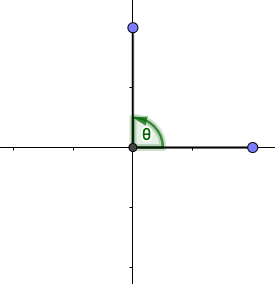
\includegraphics[scale=0.40]{images/angle-1-digital}
    \item 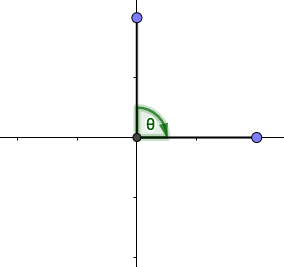
\includegraphics[scale=0.40]{images/angle-2-digital}
  \end{enumerate}  
  \end{minipage}
  \begin{minipage}{0.5\linewidth}
    \begin{enumerate}
    \item[(c)] 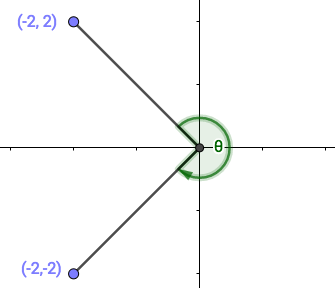
\includegraphics[scale=0.40]{images/angle-3-digital}
    \item[(d)] 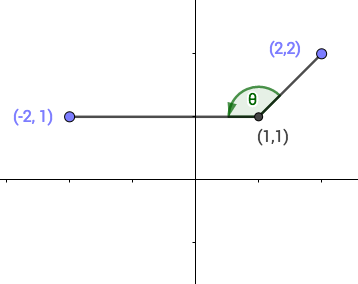
\includegraphics[scale=0.40]{images/angle-4-digital}
    \end{enumerate}
  \end{minipage}
\end{ex}
\begin{defi}
  What is the \emph{unit circle}, what is \emph{arc length}, and what
  are \emph{radians}?
\end{defi}
\vs\vs
\begin{ex}
  For the previous challenge, write down each angle in radians.  Then
  create your own drawing for the angles $\theta = \frac{\pi}{2}$,
  $\phi = -\pi$, and $\psi = 1$. (Remember that a circle with radius
  \(1\) had a circumference of \(2\pi\).)
\end{ex}
\begin{thrm}[Converting between degrees and radians]
  % this line intentionally blank
\end{thrm}
\vs\vs\vs
\begin{ex}
  Can you convert the angles $\alpha = 0^\deg$, $\beta = 270^\deg$, and $\gamma = -60^\deg$ into radians?  Can you convert the angles $\theta = \frac{\pi}{2}$, $\phi = -\pi$, and $\psi = 1$ into degrees?
\end{ex}
%%%%%%%%%%%%%%%%%%%%%%%%%%%%%%%%%%%%%%%%%%%%%%%%%%
\end{document}
